%\chapter{Theoretical Background}\label{chap:02}

\section{Production and Decay of \texorpdfstring{$t \overline{t}$}{}}

Top quark pairs ($t\overline{t}$) are dominantly produced through strong interaction in high-energy proton-proton collisions in processes such as gluon fusion (\autoref{fig:gluon-ttbar}). Once produced, the top and anti-top quarks decay almost exclusively via the weak interaction into a $W$ boson and a bottom-type quark.

\begin{figure}[H]
       \setkeys{Gin}{draft=false}
	\centering
	\fcolorbox{black}{white}{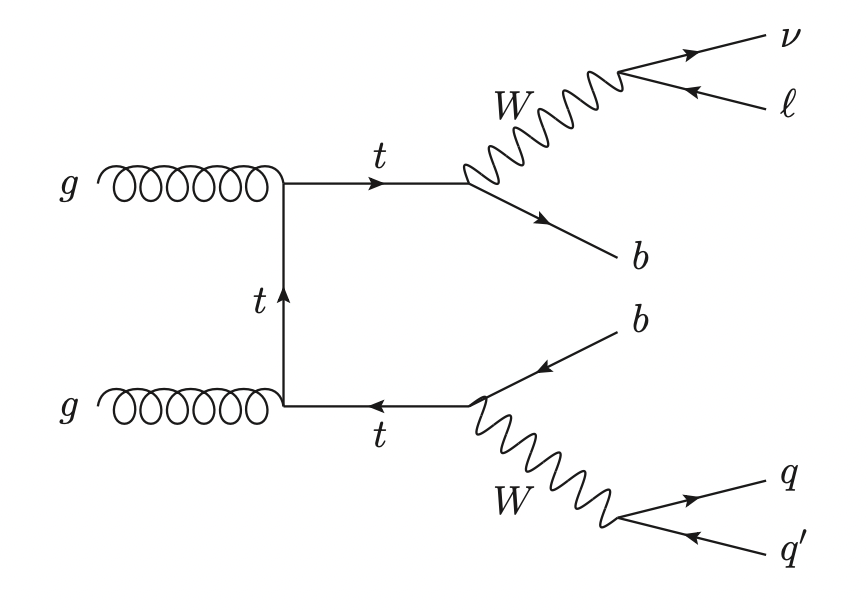
\includegraphics[scale=0.3]{images/gluon-ttbar_feynman.png}}
	\caption{Feynman diagram of gluon fusion-$t\overline{t}$ production  which later decays into lepton+jets channel.}
	\label{fig:gluon-ttbar}
\end{figure}

The decay channels of the $t\overline{t}$ pair events are thus governed by the subsequent decays of the (two) $W$ bosons, each of which can decay either hadronically (into a pair of quarks) or leptonically (into a lepton and neutrino). Decays of the $W$ boson into a different generation quark-antiquark is possible, but it is CKM supressed and these cases do not constitute an additional decay branch. In experimental analyses, each final state has its strengths and weaknesses. \\

Depending on the decay modes of the two $W$ bosons, $t\overline{t}$ events are categorized into three primary final states:


\begin{itemize}
\item \textbf{All-Hadronic Channel} ($t\overline{t}\rightarrow b\overline{b}q\overline{q}'q''\overline{q}'''$) 
In this channel, both $W$ bosons decay into quark-antiquark pairs, resulting in a final state composed solely of jets. Alongside the two $b$-jets from the top quark decays, the event contains four additional light-flavor jets from the $W$ bosons. Although this channel has the largest branching ratio (about 44\%), it suffers from significant QCD multijet background, making signal discrimination challenging.

\begin{figure}[H]
    \centering
    \begin{tikzpicture}
        \begin{feynman}
            \vertex (a1) {\(t\)};
            \vertex[right=3cm of a1] (a2);
            \vertex[right=3cm of a2] (a3){\(b\)};
            \vertex[right=1.5cm of a2] (ac);
            \vertex[above=1.5cm of ac] (c1);
            \vertex[red, above=1cm of a3] (cu){\(q\)};
            \vertex[red, above=2cm of a3] (co){\(\overline q'\)};
            \vertex[below=1cm of a1] (b1) {\(\overline t\)};
            \vertex[below=1cm of a2] (b2) ;
            \vertex[below=1cm of a3] (b3) {\(\overline b\)};
            \vertex[below=2.5cm of ac] (d1);
            \vertex[red, below=1cm of b3] (do){\(q''\)};
            \vertex[red, below=2cm of b3] (du){\(\overline q'''\)};
            \diagram* {
            (a1) -- [fermion] (a2) -- [fermion] (a3),
            (b3) -- [fermion] (b2) -- [fermion] (b1),
            (c1) -- [boson, edge label=\(W^{+}\)] (a2),
            (d1) -- [boson, edge label=\(W^{-}\)] (b2),
            (co) -- [red, fermion] (c1) -- [red, fermion] (cu),
            (du) -- [red, fermion] (d1) -- [red, fermion] (do),
            };
            \draw [decoration={brace}, decorate] (b1.south west) -- (a1.north west)
            node [pos=0.5, left];
        \end{feynman}
    \end{tikzpicture}  
\caption{Feynman diagram for the Fully Hadronic decay channel.}
\end{figure}

\item \textbf{Lepton+Jets Channel} ($t\overline{t}\rightarrow b\overline{b} \nu \overline{l} q\overline{q}'$)
Here, one $W$ decays leptonically and the other hadronically. The final state includes one charged lepton (electron or muon), missing transverse energy from the undetected neutrino, two light-flavor jets, and two $b$-jets. This channel offers a balance between background suppression and signal yield, with a branching fraction of about 44\% (all lepton flavors). The presence of a high-$p_t$ (transverse momentum) lepton and $E^{miss}_T$ (missing transverse energy) makes it particularly suitable for triggering and analysis.

\begin{figure}[H]
    \centering
    \begin{tikzpicture}
        \begin{feynman}
            \vertex (a1) {\(t\)};
            \vertex[right=3cm of a1] (a2);
            \vertex[right=3cm of a2] (a3){\(b\)};
            \vertex[right=1.5cm of a2] (ac);
            \vertex[above=1.5cm of ac] (c1);
            \vertex[blue, above=1cm of a3] (cu){\(\nu\)};
            \vertex[blue, above=2cm of a3] (co){\(\overline l\)};
            \vertex[below=1cm of a1] (b1) {\(\overline t\)};
            \vertex[below=1cm of a2] (b2) ;
            \vertex[below=1cm of a3] (b3) {\(\overline b\)};
            \vertex[below=2.5cm of ac] (d1);
            \vertex[red, below=1cm of b3] (do){\(q\)};
            \vertex[red, below=2cm of b3] (du){\(\overline q'\)};
            \diagram* {
            (a1) -- [fermion] (a2) -- [fermion] (a3),
            (b3) -- [fermion] (b2) -- [fermion] (b1),
            (c1) -- [boson, edge label=\(W^{+}\)] (a2),
            (d1) -- [boson, edge label=\(W^{-}\)] (b2),
            (co) -- [blue, fermion] (c1) -- [blue, fermion] (cu),
            (du) -- [red, fermion] (d1) -- [red, fermion] (do),
            };
            \draw [decoration={brace}, decorate] (b1.south west) -- (a1.north west)
            node [pos=0.5, left];
        \end{feynman}
    \end{tikzpicture}  
\caption{Feynman diagram for the Lepton + Jets decay channel.}
\end{figure}

\newpage

\item \textbf{Dileptonic Channel} ($t\overline{t}\rightarrow b\overline{b} \nu \overline{l} l'\overline{\nu}'$)
In the dilepton channel, both $W$ bosons decay leptonically, leading to two oppositely charged leptons (electrons or muons), missing transverse energy from the neutrinos, and two $b$-jets. This channel is the cleanest in terms of background (particularly from QCD), but it has the lowest branching fraction (about 11\% ). The reconstruction of the event is more difficult due to the presence of two neutrinos, which escape detection.


\begin{figure}[H]
    \centering
    \begin{tikzpicture}
        \begin{feynman}
            \vertex (a1) {\(t\)};
            \vertex[right=3cm of a1] (a2);
            \vertex[right=3cm of a2] (a3){\(b\)};
            \vertex[right=1.5cm of a2] (ac);
            \vertex[above=1.5cm of ac] (c1);
            \vertex[blue, above=1cm of a3] (cu){\(\nu\)};
            \vertex[blue, above=2cm of a3] (co){\(\overline l\)};
            \vertex[below=1cm of a1] (b1) {\(\overline t\)};
            \vertex[below=1cm of a2] (b2) ;
            \vertex[below=1cm of a3] (b3) {\(\overline b\)};
            \vertex[below=2.5cm of ac] (d1);
            \vertex[blue, below=1cm of b3] (do){\(l'\)};
            \vertex[blue, below=2cm of b3] (du){\(\overline \nu'\)};
            \diagram* {
            (a1) -- [fermion] (a2) -- [fermion] (a3),
            (b3) -- [fermion] (b2) -- [fermion] (b1),
            (c1) -- [boson, edge label=\(W^{+}\)] (a2),
            (d1) -- [boson, edge label=\(W^{-}\)] (b2),
            (co) -- [blue, fermion] (c1) -- [blue, fermion] (cu),
            (du) -- [blue, fermion] (d1) -- [blue, fermion] (do),
            };
            \draw [decoration={brace}, decorate] (b1.south west) -- (a1.north west)
            node [pos=0.5, left];
        \end{feynman}
    \end{tikzpicture}  
\caption{Feynman diagram for the Dileptonic decay channel:}
\end{figure}

\end{itemize}


\section{Probing Beyond the Standard Model: \texorpdfstring{$Z' \rightarrow t\overline{t}$}{}}

The analysis of the \( Z' \rightarrow t\bar{t} \) process is a direct probe of physics beyond the Standard Model (BSM) in the search for a heavy BSM boson. Many BSM theories predict the existence of additional neutral gauge bosons (\( Z' \)) or other heavy states that preferentially decay into top-quark pairs due to their large Yukawa coupling. The kinematic properties of high-mass resonance $t\bar{t}$ production in proton-proton collisions produce distinct signatures in the ATLAS detector. Some examples are large transverse momenta, boosted topologies, collimated jets from hadronic decays of boosted quarks and large missing transverse energy due to leptonic decays.\\

In this analysis we will leverage the reconstruction of invariant mass distributions of \( m_{t\bar{t}} \), to search for a resonance bump above the falling Standard Model background. A statistically significant bump in the \( m_{t\bar{t}} \) spectrum could indicate the presence of a new heavy particle. Limits on the production cross section times branching ratio of a hypothetical \( Z' \) boson are derived as a function of its mass. This enables constraints to be placed on specific BSM models or, in the case of a signal-like excess, motivates further investigation.